\documentclass[11pt,a4paper]{beamer}
\usepackage[latin1]{inputenc}
\usepackage[dutch]{babel}

\usepackage[absolute,overlay]{textpos}
  \setlength{\TPHorizModule}{1mm}
  \setlength{\TPVertModule}{1mm}

\author{Zeus WPI}

\definecolor{gray}{RGB}{56,56,56}

\begin{document}

% Main logo
\setbeamercolor{background canvas}{bg=gray}
\begin{frame}
    
\includegraphics[width=\textwidth]{zeus_logo_oranje.pdf}\\[5mm]

    \hfill \textcolor{white}{- by Noctua \&\& Procrat}

    \note{Wij komen Zeus-WPI voorstellen. Zeus is een werkgroep van studenten,
    voor mensen uit de informatica, en al de rest die geinteresseerd is.}
\end{frame}

% Who
\begin{frame}
    \textcolor{white}{
        {\huge Activiteiten:}\\[1mm]
        {\LARGE
            | Informatica-gerelateerde talks\\[1mm]
            | Ontspannende geekactiviteiten\\[3mm]
        }
        {\huge Projecten:}\\[1mm]
        {\LARGE
            | Hydra \\[1mm]
            | 12urenloop \\[1mm]
        }
    }

    \note{Zeus voorziet eigenlijk 3 dingen voor informatici en geinteresseerden.
        Enerzijds organizeren we activiteiten, die varieren van echte lessen tot
        ontspannen prutsen. Anderzijds werken we met de leden aan diverse
        projecten zoals Hydra en het automatische telsysteem van de 12-urenloop.
    Tenslotte zorgen we ook voor een gezellige sfeer onder mede-geeks.}
\end{frame}

% Activities
\begin{frame}

    \begin{center}
        \textcolor{white}{\Huge{Activiteiten}}\\[3mm]
    \end{center}

    \note{Ik zou nu liefst wat dieper ingaan op de activiteiten die wij zoal
    doen.}

    \setlength{\fboxsep}{0pt}
    \setlength{\fboxrule}{1pt}

    \pause
    \begin{textblock}{20}(3,45)
        \visible<2->{\fbox{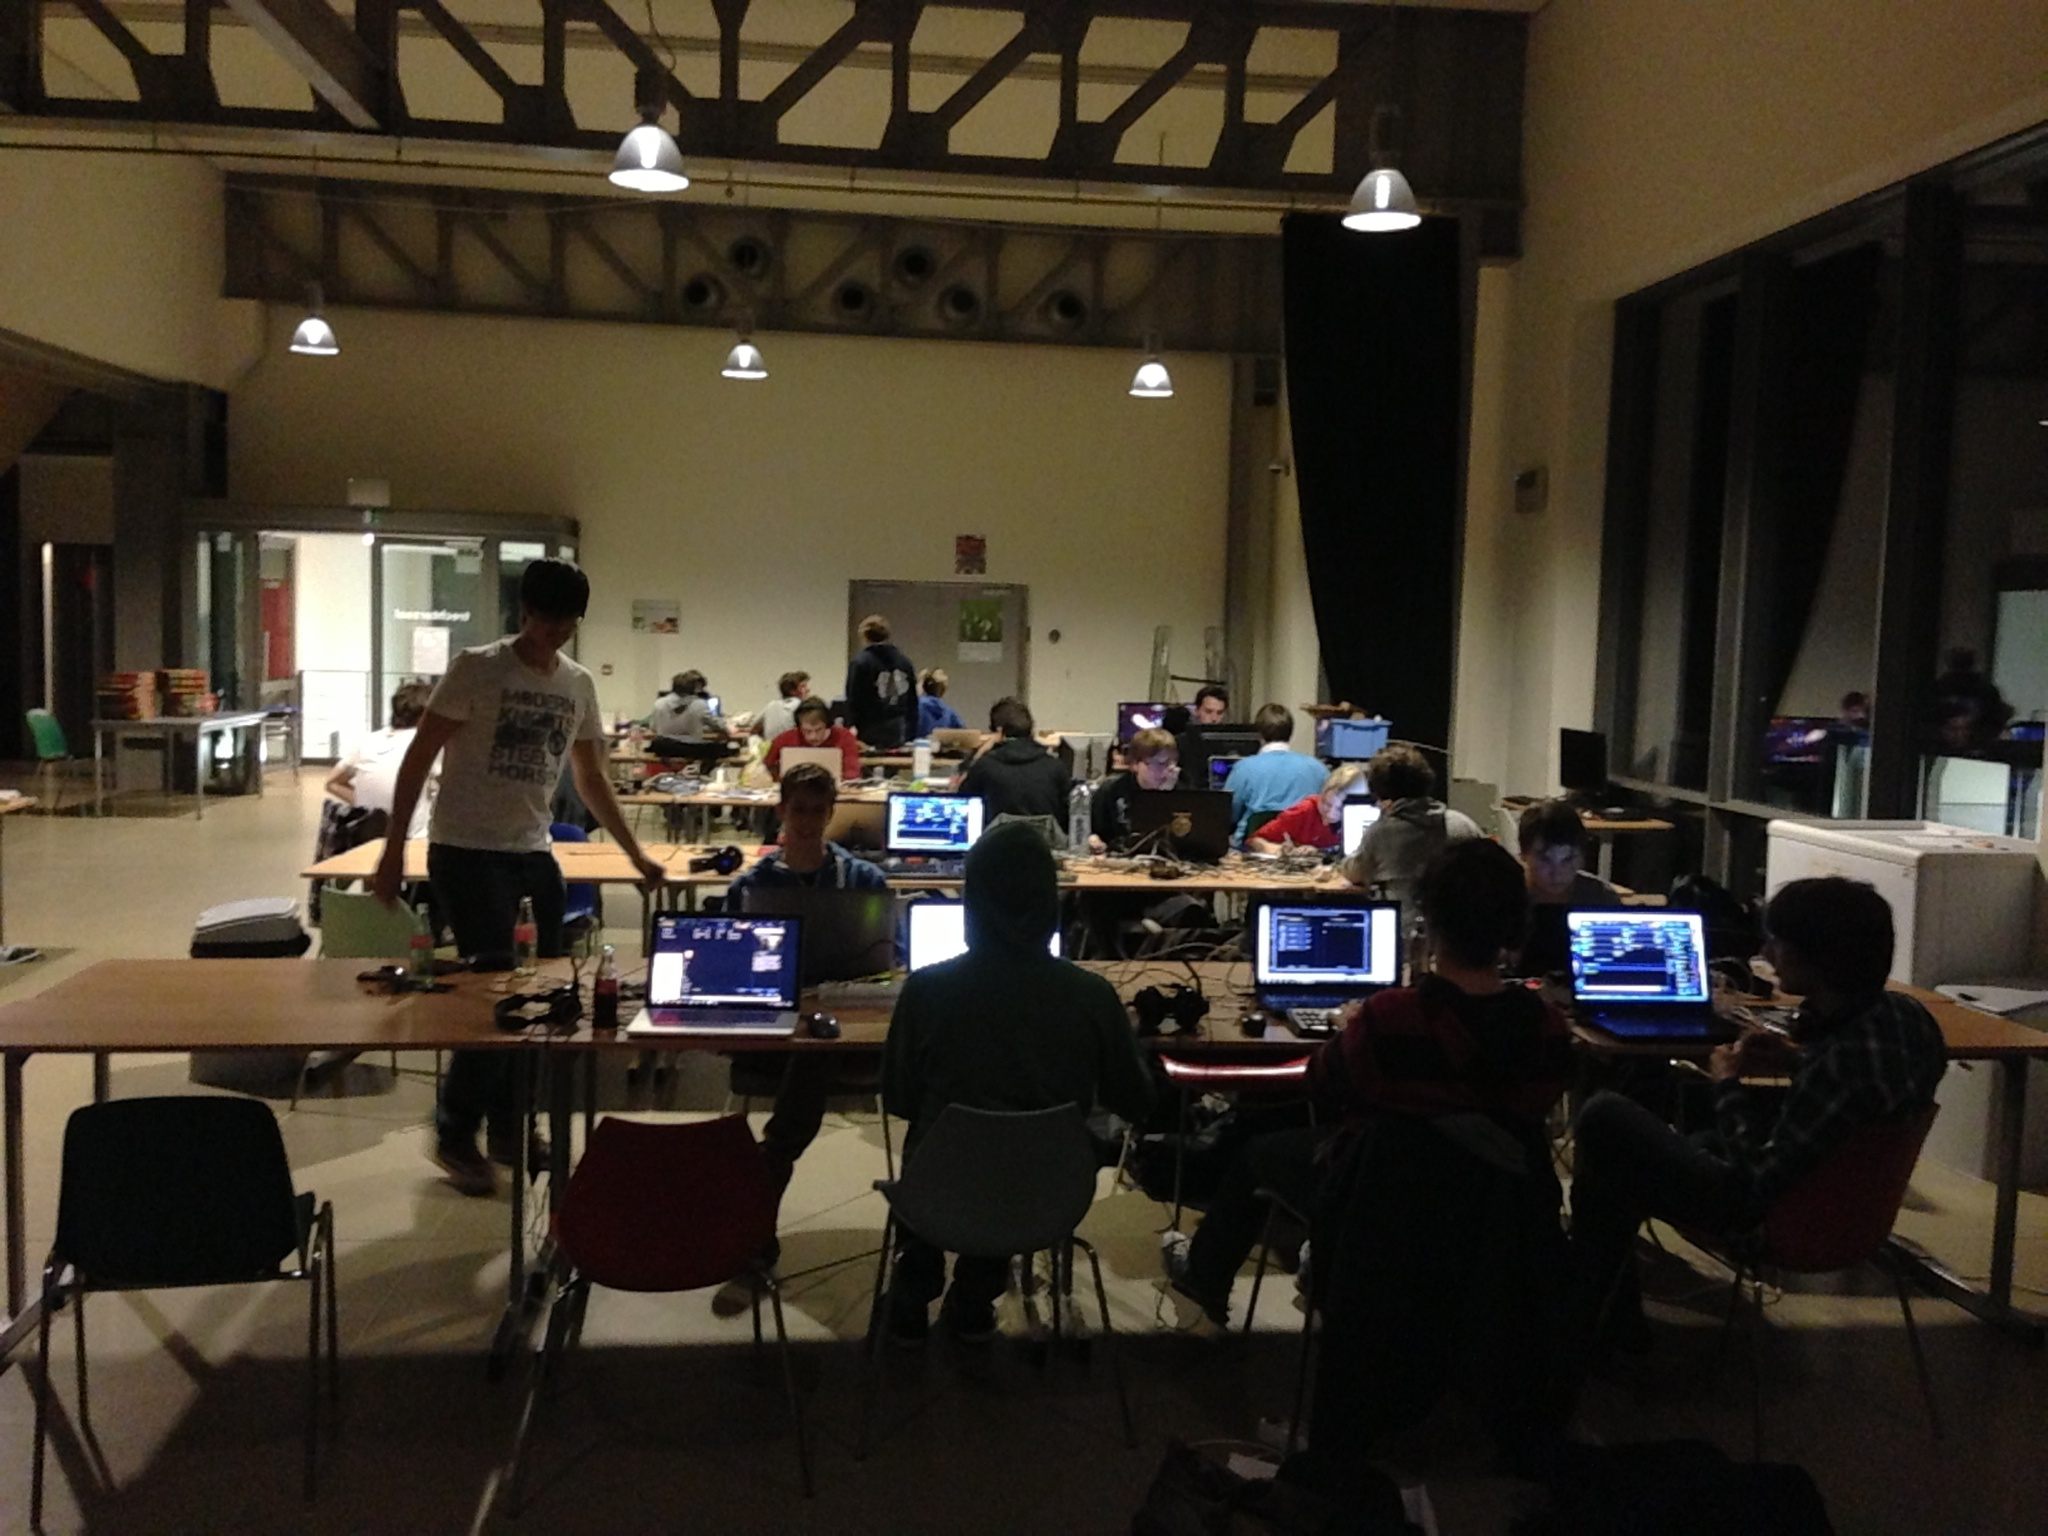
\includegraphics[width=180pt]{activiteit_lan.jpg}}}
    \end{textblock}

    \note<2->{Die zijn niet allemaal even serieus. Zo hebben we dit jaar al een
        24-uren-LAN-party ingelast, omdat die van vorig jaar (waar je hier de
    foto van ziet) goed gelukt was.}

    \pause
    \begin{textblock}{20}(32,20)
        \visible<3->{\fbox{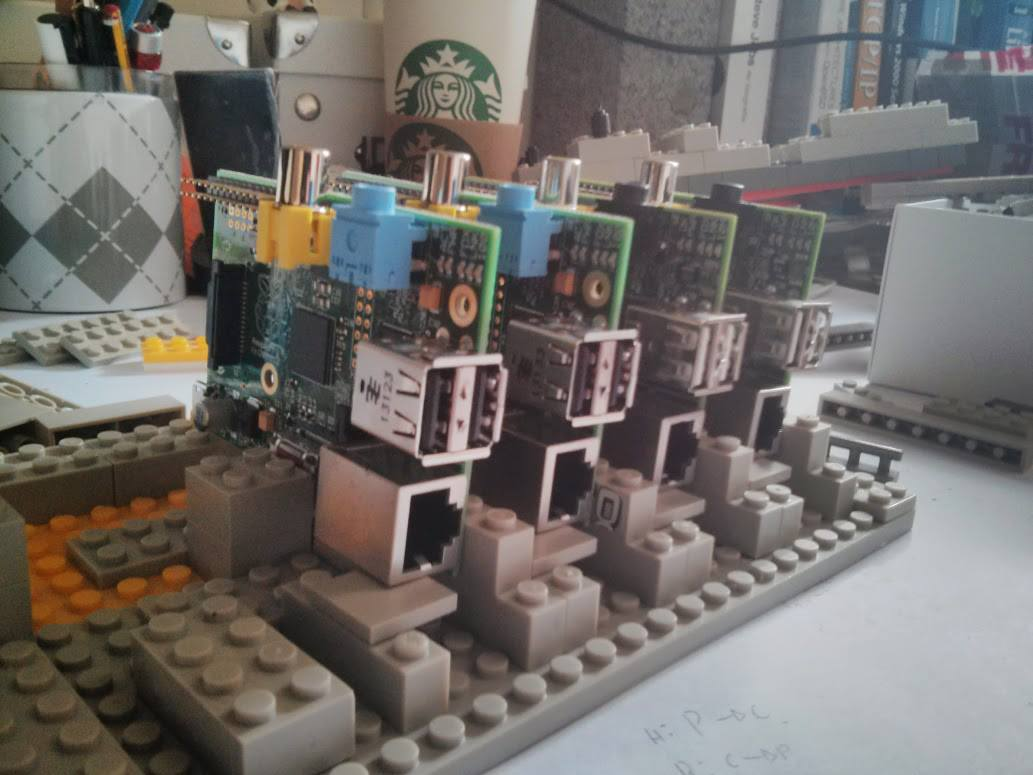
\includegraphics[width=180pt]{arm-cluster.jpg}}}
    \end{textblock}

    \note<3->{Verder zouden we dit jaar ook een herhaling van de hardware-avond
        houden. Dat is eigenlijk een avondje prutsen met lego, raspberry-pi's en
    een paar circuitjes.}


    \pause
    \begin{textblock}{20}(61,3)
        \visible<4->{\fbox{\includegraphics[width=180pt]{kelder1.jpeg}}}
    \end{textblock}

    \note<4->{Voor wie liever met software bezig is zijn er de code-nights, die
        bijna elke week doorgaan. Dan werken we onder andere aan de projecten
        die we daarnet noemden, of aan dingen van jezelf. Natuurlijk zit er op
    andere avonden ook vaak gewoon volk te werken.}

    \pause
    \begin{textblock}{20}(10,10)
        \visible<5->{\fbox{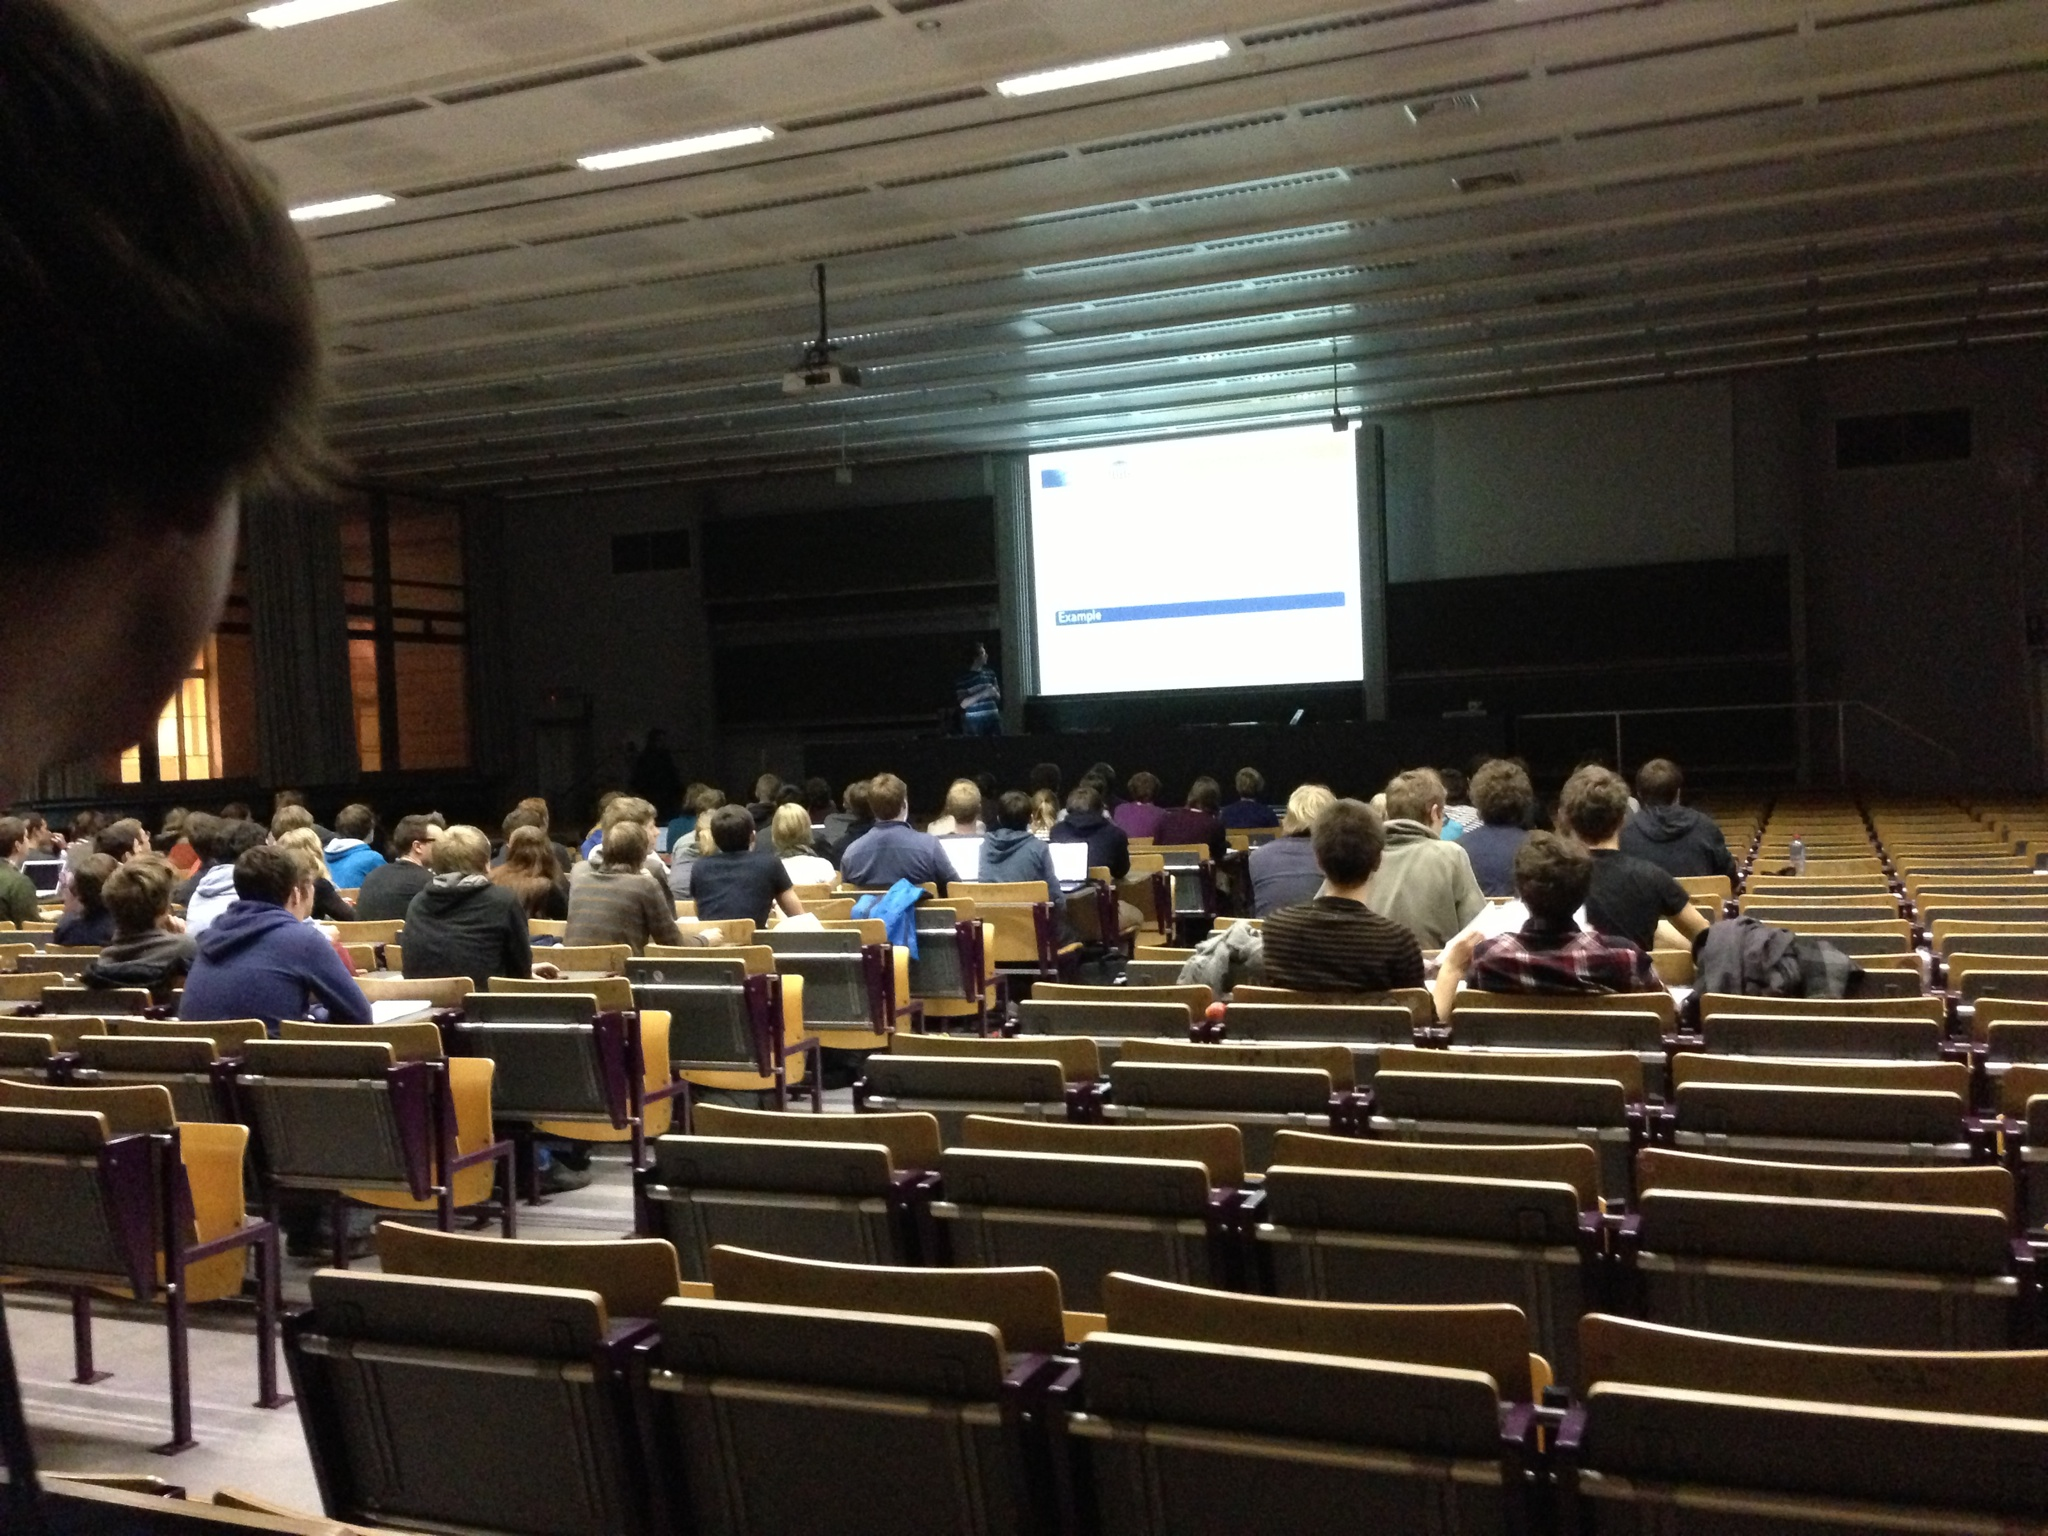
\includegraphics[width=180pt]{activiteit_latex.jpg}}}
    \end{textblock}

    \note<5->{Natuurlijk kunnen de meeste mensen hier nog niet genoeg coden om
        veel bijdrage te leveren bij die projecten. Ge kunt wachten tot ge in de
        lessen hebt leren programmeren, maar wie haas heeft kan altijd komen
        kijken naar enkele van onze informele lessen. Vorig jaar waren er een
    git-les en python-les, dit is een foto van de latex-les.}

    \pause
    \begin{textblock}{20}(54,50)
        \visible<6->{\fbox{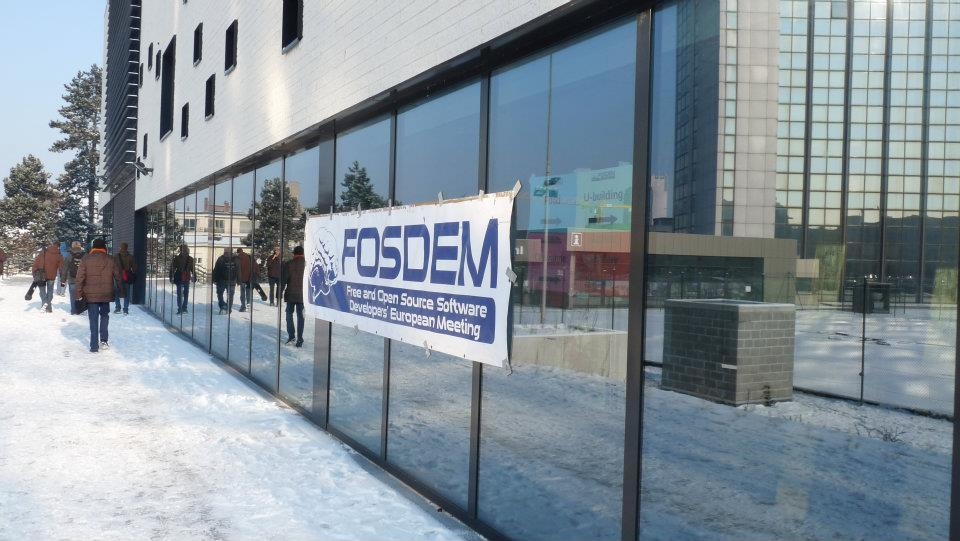
\includegraphics[width=180pt]{activiteit_fosdem.jpg}}}
    \end{textblock}

    \note<6->{Soms verlaten we onze eigen domeinen echter, en trekken we naar
        grotere evenementen, zoals FOSDEM of de Vlaamse Programmeerwedstrijd.
        Vorig jaar hebben we ook eens de parking overgestoken om de
    supercomputer te aanschouwen.}

\end{frame}

% Where - Projects
\begin{frame}
    \begin{center}
        \textcolor{white}{\Huge{Zeus Basement}}\\[3mm]
        \hspace*{-230pt}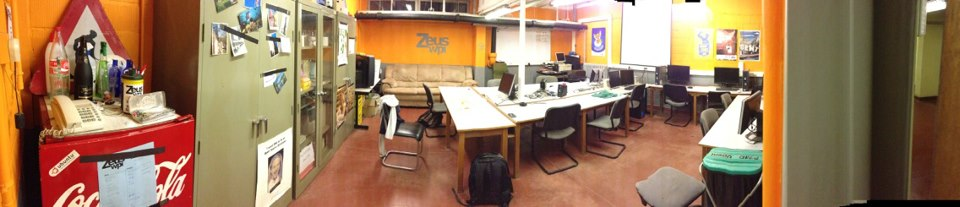
\includegraphics[width=700pt]{kelder.jpg}

        \textcolor{white}{51.023102,3.710265 | Verdieping -1}

        \textcolor{white}{irc://wina.ugent.be:6667/\#zeus}
    \end{center}
    \begin{textblock}{20}(3,57)
        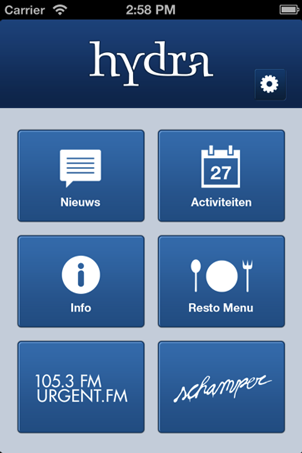
\includegraphics[width=70pt]{hydra-iphone.png}
    \end{textblock}

    \note{Voor wie zich nu zou afvragen waar dit zich allemaal afspeelt: wij
        hebben hier beneden een gezellige kelder, waar er tussen de lessen door
        en 's avonds vaak volk zit. Met voorstellen van activiteiten en vragen
        over geeky knowledge kunt ge dus ook steeds naar daar komen. Wie kans
        wil maken om 20 euro's te winnen, kan straks al eens langs komen om
    de Hydra-app te installeren.}

    \note{Ge zijt trouwens ook allemaal welkom op onze inleidende activiteit, ge
        zult ons wel zien hangen op de gemeenschappelijke posters. Maar
    informatie erover vogt nog.}
\end{frame}

\end{document}
